\documentclass{article}
\usepackage[paperwidth=86cm,paperheight=64cm,margin=0.8cm]{geometry}
\usepackage{fontspec}
\usepackage{amsmath}
\usepackage{unicode-math}
\setmainfont{texgyreheros}[Extension=.otf,UprightFont=*-regular,BoldFont=*-bold,ItalicFont=*-italic,BoldItalicFont=*-bolditalic]
\setmathfont{texgyrepagella-math.otf}
\usepackage[table]{xcolor}
\usepackage{tikz}
\usetikzlibrary{arrows.meta,positioning,calc,backgrounds}
\usepackage{adjustbox}
\pagestyle{empty}

\definecolor{ink}{HTML}{14213D}
\definecolor{trust}{HTML}{2F7A4F}
\definecolor{curious}{HTML}{C8611E}
\definecolor{untrusted}{HTML}{A23B3B}
\definecolor{chan}{HTML}{2F5F98}
\definecolor{soft}{HTML}{F3EFE6}
\definecolor{softblue}{HTML}{E6EEF8}
\definecolor{softgreen}{HTML}{E4F1E8}
\definecolor{softred}{HTML}{F6E3E1}
\definecolor{grey}{HTML}{6B7280}
\definecolor{bankc}{HTML}{1F6F8B}
\definecolor{keyc}{HTML}{8E2C6E}
\definecolor{gold}{HTML}{9A6B00}
\definecolor{softgold}{HTML}{FBF3DC}

\newcommand{\bk}{\tikz[baseline=(c.base)]\node[fill=bankc,text=white,rounded corners=1pt,inner sep=1.4pt,font=\bfseries\fontsize{7}{7}\selectfont] (c) {bank};}
\newcommand{\ek}{\tikz[baseline=(c.base)]\node[fill=keyc,text=white,rounded corners=1pt,inner sep=1.4pt,font=\bfseries\fontsize{7}{7}\selectfont] (c) {enclave};}
\newcommand{\pp}[1]{\tikz[baseline=(c.base)]\node[draw=ink,text=ink,rounded corners=1pt,inner sep=1.2pt,font=\bfseries\fontsize{7}{7}\selectfont] (c) {#1};}
\newcommand{\disk}[1]{\tikz[baseline=(c.base)]\node[fill=grey!20,draw=grey,text=ink,rounded corners=1pt,inner sep=1.4pt,font=\ttfamily\fontsize{7.6}{7.6}\selectfont] (c) {\detokenize{#1}};}
\newcommand{\kk}[1]{\tikz[baseline=(c.base)]\node[fill=softgold,draw=gold,text=gold,rounded corners=1pt,inner sep=1.4pt,font=\bfseries\fontsize{7.4}{7.4}\selectfont] (c) {#1};}
\newcommand{\num}[1]{\tikz[baseline=(c.base)]\node[circle,fill=ink,text=white,inner sep=1pt,font=\bfseries\fontsize{7.6}{7.6}\selectfont] (c) {#1};}
\newcommand{\cd}[1]{{\ttfamily\detokenize{#1}}}
\newcommand{\hd}[1]{{\bfseries #1}}
\newcommand{\sm}{\fontsize{9.8}{11.8}\selectfont}
\newcommand{\xs}{\fontsize{8.8}{10.6}\selectfont}

\tikzset{
  lane/.style={draw=grey!60,dashed,line width=0.6pt},
  head/.style={draw,rounded corners=3pt,line width=1.1pt,font=\sm\bfseries,minimum width=6.4cm,minimum height=1.3cm,align=center},
  note/.style={draw=grey,fill=white,rounded corners=2pt,align=left,inner sep=4pt,font=\xs},
  file/.style={draw=grey,fill=grey!8,align=left,inner sep=4pt,font=\xs,double,double distance=1pt},
  arr/.style={-{Stealth[length=7pt]},line width=1pt,ink},
  sarr/.style={-{Stealth[length=7pt]},line width=1pt,chan},
  darr/.style={-{Stealth[length=7pt]},line width=0.9pt,grey,dashed},
  msg/.style={font=\xs,fill=white,inner sep=1.5pt,align=center},
  phase/.style={font=\sm\bfseries,text=grey,anchor=south west,inner sep=2pt},
}

\newcommand{\call}[6][arr]{%
  \node[msg,anchor=north,text width=#4] (#6l) at ($(cur -| #2)!0.5!(cur -| #3)$) {#5};
  \coordinate (#6) at ($(#6l.south)+(0,-0.14)$);
  \draw[#1] (#6 -| #2) -- (#6 -| #3);
  \coordinate (cur) at ($(#6)+(0,-0.4)$);
}
\newcommand{\after}[2][0.35]{\coordinate (cur) at ($(#2.south)+(0,-#1)$);}
\newcommand{\aftertwo}[3][0.35]{\path let \p1=(#2.south), \p2=(#3.south) in coordinate (cur) at (0,{min(\y1,\y2)-#1 cm});}
\newcommand{\phaseline}[1]{%
  \coordinate (cur) at ($(cur)+(0,-0.55)$);
  \draw[grey!45,line width=0.8pt] ($(cur -| L0)+(0,-0.1)$) -- ($(cur -| L9)+(0,-0.1)$);
  \node[phase] at ($(cur -| L0)+(0,-0.05)$) {#1};
  \coordinate (cur) at ($(cur)+(0,-0.75)$);
}

\begin{document}
\hyphenpenalty=10000\exhyphenpenalty=10000
\noindent
\begin{adjustbox}{max width=\linewidth,max totalheight=0.98\textheight,center}
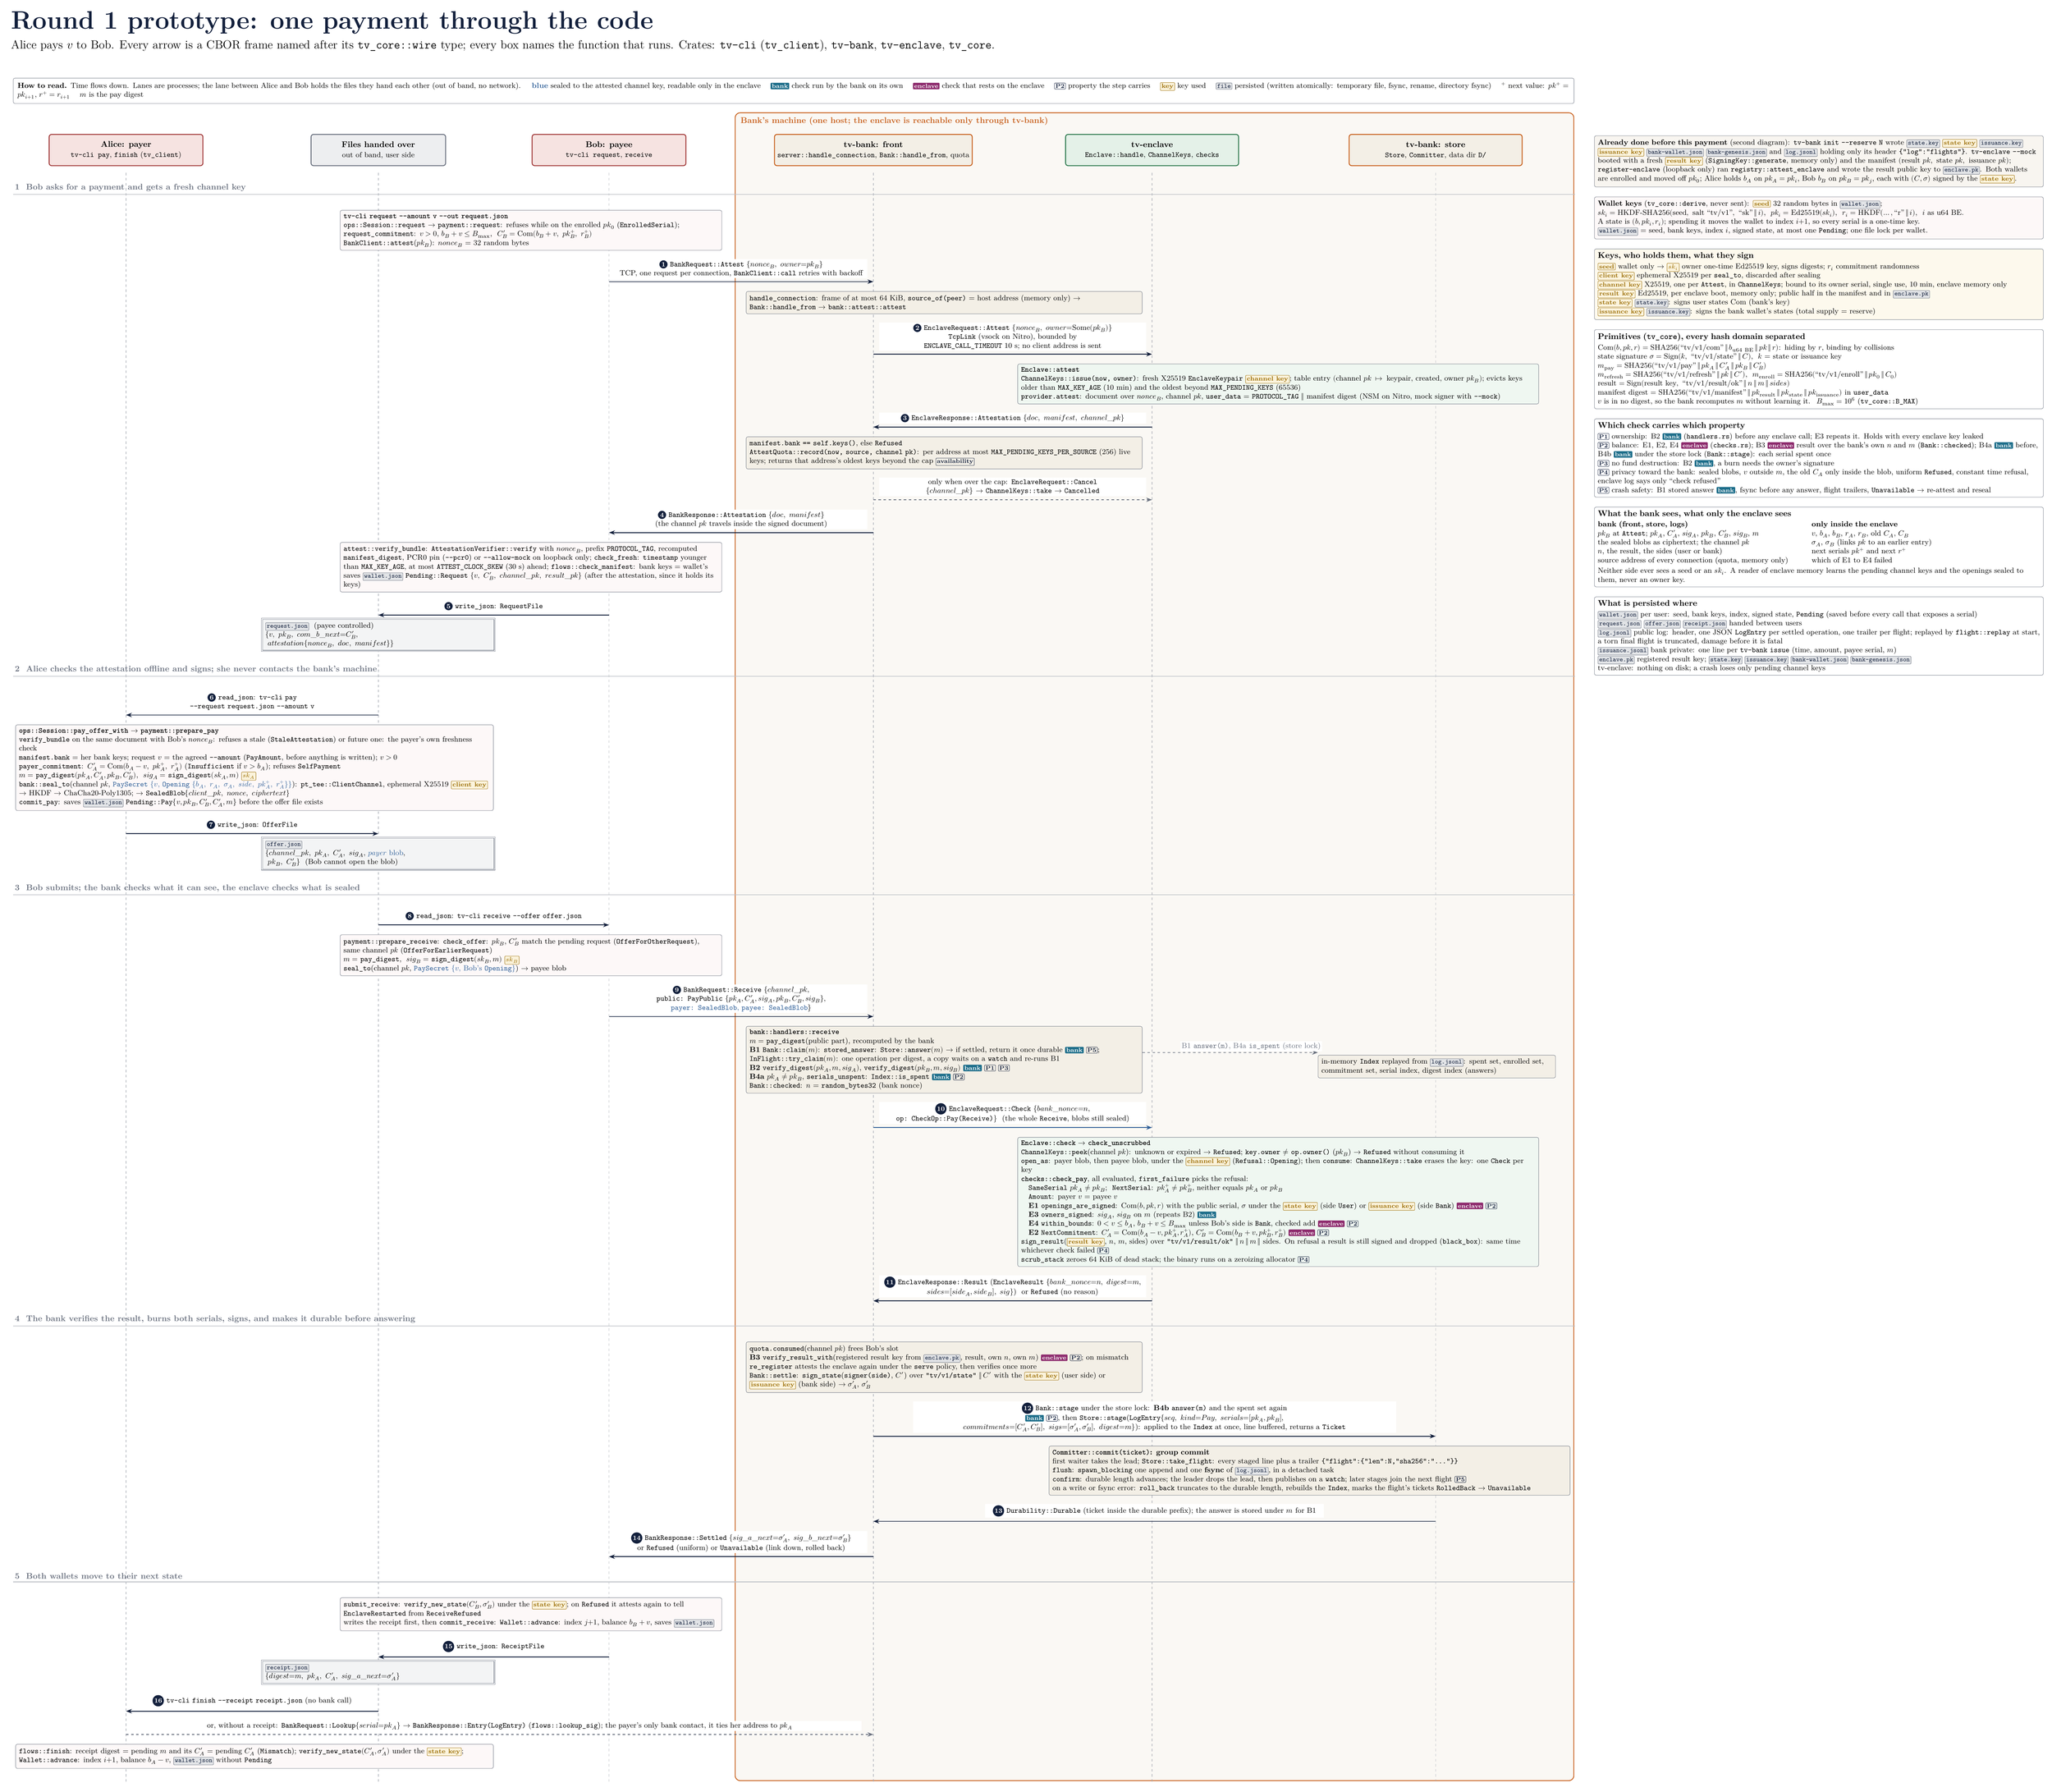
\begin{tikzpicture}[x=1cm,y=1cm]

\def\xA{4.9}\def\xF{15.4}\def\xB{25.0}\def\xK{36.0}\def\xE{47.6}\def\xS{59.4}
\coordinate (LA) at (\xA,0);
\coordinate (LF) at (\xF,0);
\coordinate (LB) at (\xB,0);
\coordinate (LK) at (\xK,0);
\coordinate (LE) at (\xE,0);
\coordinate (LS) at (\xS,0);
\coordinate (L0) at (0.2,0);
\coordinate (L9) at (65.2,0);

\node[anchor=north west,align=left] at (0,58.2) {{\bfseries\fontsize{30}{34}\selectfont\color{ink} Round 1 prototype: one payment through the code}\\[6pt]{\fontsize{14}{17}\selectfont Alice pays $v$ to Bob. Every arrow is a CBOR frame named after its \cd{tv_core::wire} type; every box names the function that runs. Crates: \cd{tv-cli} (\cd{tv_client}), \cd{tv-bank}, \cd{tv-enclave}, \cd{tv_core}.}};

\node[anchor=north west,align=left,font=\xs,draw=grey,rounded corners=2pt,inner sep=5pt,text width=64.6cm] at (0.2,55.3) {
\hd{How to read.} Time flows down. Lanes are processes; the lane between Alice and Bob holds the files they hand each other (out of band, no network). \quad {\color{chan}\textbf{blue}} sealed to the attested channel key, readable only in the enclave \quad \bk{} check run by the bank on its own \quad \ek{} check that rests on the enclave \quad \pp{P2} property the step carries \quad \kk{key} key used \quad \disk{file} persisted (written atomically: temporary file, fsync, rename, directory fsync) \quad $^{+}$ next value: $pk^{+}=pk_{i+1}$, $r^{+}=r_{i+1}$ \quad $m$ is the pay digest};

\node[head,draw=untrusted,fill=softred] (hA) at (\xA,52.3) {Alice: payer\\{\xs\mdseries\cd{tv-cli pay}, \cd{finish} (\cd{tv_client})}};
\node[head,draw=grey,fill=grey!12,minimum width=5.6cm] (hF) at (\xF,52.3) {Files handed over\\{\xs\mdseries out of band, user side}};
\node[head,draw=untrusted,fill=softred] (hB) at (\xB,52.3) {Bob: payee\\{\xs\mdseries\cd{tv-cli request}, \cd{receive}}};
\node[head,draw=curious,fill=soft,minimum width=7.2cm] (hK) at (\xK,52.3) {tv-bank: front\\{\xs\mdseries\cd{server::handle_connection}, \cd{Bank::handle_from}, quota}};
\node[head,draw=trust,fill=softgreen,minimum width=7.2cm] (hE) at (\xE,52.3) {tv-enclave\\{\xs\mdseries\cd{Enclave::handle}, \cd{ChannelKeys}, \cd{checks}}};
\node[head,draw=curious,fill=soft,minimum width=7.2cm] (hS) at (\xS,52.3) {tv-bank: store\\{\xs\mdseries\cd{Store}, \cd{Committer}, data dir \cd{D/}}};

\coordinate (top) at (0,51.35);
\coordinate (cur) at (0,51.1);


\phaseline{1 \ Bob asks for a payment and gets a fresh channel key}

\node[note,anchor=north east,text width=15.6cm,fill=softred!25] (b1) at ($(cur -| LB)+(4.7,0)$) {\hd{\cd{tv-cli request --amount v --out request.json}}\\
\cd{ops::Session::request} $\to$ \cd{payment::request}: refuses while on the enrolled $pk_0$ (\cd{EnrolledSerial}); \cd{request_commitment}: $v>0$, $b_B+v\le B_{\max}$, \ $C_B'=\mathrm{Com}(b_B+v,\ pk_B^{+},\ r_B^{+})$\\
\cd{BankClient::attest}($pk_B$): $nonce_B$ = 32 random bytes};
\after{b1}
\call{LB}{LK}{10.4cm}{\num{1} \cd{BankRequest::Attest} $\{nonce_B,\ owner{=}pk_B\}$\\ TCP, one request per connection, \cd{BankClient::call} retries with backoff}{a1}

\node[note,anchor=north west,text width=16.2cm,fill=soft] (k1) at ($(cur -| LK)+(-5.3,0)$) {\cd{handle_connection}: frame of at most 64 KiB, \cd{source_of(peer)} = host address (memory only) $\to$ \cd{Bank::handle_from} $\to$ \cd{bank::attest::attest}};
\after{k1}
\call{LK}{LE}{11cm}{\num{2} \cd{EnclaveRequest::Attest} $\{nonce_B,\ owner{=}\mathrm{Some}(pk_B)\}$\\ \cd{TcpLink} (vsock on Nitro), bounded by \cd{ENCLAVE_CALL_TIMEOUT} 10 s; no client address is sent}{a2}

\node[note,anchor=north west,text width=21.4cm,fill=softgreen!60] (e1) at ($(cur -| LE)+(-5.6,0)$) {\hd{\cd{Enclave::attest}}\\
\cd{ChannelKeys::issue(now, owner)}: fresh X25519 \cd{EnclaveKeypair} \kk{channel key}; table entry $(\text{channel } pk \mapsto \text{keypair, created, owner } pk_B)$; evicts keys older than \cd{MAX_KEY_AGE} (10 min) and the oldest beyond \cd{MAX_PENDING_KEYS} (65536)\\
\cd{provider.attest}: document over $nonce_B$, channel $pk$, \cd{user_data} = \cd{PROTOCOL_TAG} $\|$ manifest digest (NSM on Nitro, mock signer with \cd{--mock})};
\after{e1}
\call{LE}{LK}{11cm}{\num{3} \cd{EnclaveResponse::Attestation} $\{doc,\ manifest,\ channel\_pk\}$}{a3}

\node[note,anchor=north west,text width=16.2cm,fill=soft] (k2) at ($(cur -| LK)+(-5.3,0)$) {\cd{manifest.bank == self.keys()}, else \cd{Refused}\\
\cd{AttestQuota::record(now, source, channel pk)}: per address at most \cd{MAX_PENDING_KEYS_PER_SOURCE} (256) live keys; returns that address's oldest keys beyond the cap \pp{availability}};
\after{k2}
\call[darr]{LK}{LE}{11cm}{only when over the cap: \cd{EnclaveRequest::Cancel} $\{channel\_pk\}$ $\to$ \cd{ChannelKeys::take} $\to$ \cd{Cancelled}}{a3b}
\call{LK}{LB}{10.4cm}{\num{4} \cd{BankResponse::Attestation} $\{doc,\ manifest\}$\\ (the channel $pk$ travels inside the signed document)}{a4}

\node[note,anchor=north east,text width=15.6cm,fill=softred!25] (b2) at ($(cur -| LB)+(4.7,0)$) {\cd{attest::verify_bundle}: \cd{AttestationVerifier::verify} with $nonce_B$, prefix \cd{PROTOCOL_TAG}, recomputed \cd{manifest_digest}, PCR0 pin (\cd{--pcr0}) or \cd{--allow-mock} on loopback only; \cd{check_fresh}: \cd{timestamp} younger than \cd{MAX_KEY_AGE}, at most \cd{ATTEST_CLOCK_SKEW} (30 s) ahead; \cd{flows::check_manifest}: bank keys = wallet's\\
saves \disk{wallet.json} \cd{Pending::Request} $\{v,\ C_B',\ channel\_pk,\ result\_pk\}$ (after the attestation, since it holds its keys)};
\after{b2}
\call{LB}{LF}{8.8cm}{\num{5} \cd{write_json}: \cd{RequestFile}}{a5}
\node[file,anchor=north,text width=9.4cm] (f1) at ($(a5 -| LF)+(0,-0.15)$) {\disk{request.json} \ (payee controlled)\\$\{v,\ pk_B,\ com\_b\_next{=}C_B',$\\ $\ attestation\{nonce_B,\ doc,\ manifest\}\}$};
\after[0.4]{f1}

\phaseline{2 \ Alice checks the attestation offline and signs; she never contacts the bank's machine}

\call{LF}{LA}{8.8cm}{\num{6} \cd{read_json}: \cd{tv-cli pay --request request.json --amount v}}{a6}
\node[note,anchor=north west,text width=19.6cm,fill=softred!25] (al1) at ($(cur -| L0)+(0.1,0)$) {\hd{\cd{ops::Session::pay_offer_with} $\to$ \cd{payment::prepare_pay}}\\
\cd{verify_bundle} on the same document with Bob's $nonce_B$: refuses a stale (\cd{StaleAttestation}) or future one: the payer's own freshness check\\
\cd{manifest.bank} = her bank keys; request $v$ = the agreed \cd{--amount} (\cd{PayAmount}, before anything is written); $v>0$\\
\cd{payer_commitment}: $C_A'=\mathrm{Com}(b_A-v,\ pk_A^{+},\ r_A^{+})$ (\cd{Insufficient} if $v>b_A$); refuses \cd{SelfPayment}\\
$m=$ \cd{pay_digest}$(pk_A, C_A', pk_B, C_B')$, \ $sig_A=$ \cd{sign_digest}$(sk_A, m)$ \kk{$sk_A$}\\
\cd{bank::seal_to}(channel $pk$, {\color{chan}\cd{PaySecret} $\{v,$ \cd{Opening} $\{b_A,\ r_A,\ \sigma_A,\ side,\ pk_A^{+},\ r_A^{+}\}\}$}): \cd{pt_tee::ClientChannel}, ephemeral X25519 \kk{client key} $\to$ HKDF $\to$ ChaCha20-Poly1305; $\to$ \cd{SealedBlob}$\{client\_pk,\ nonce,\ ciphertext\}$\\
\cd{commit_pay}: saves \disk{wallet.json} \cd{Pending::Pay}$\{v, pk_B, C_B', C_A', m\}$ before the offer file exists};
\after{al1}
\call{LA}{LF}{8.8cm}{\num{7} \cd{write_json}: \cd{OfferFile}}{a7}
\node[file,anchor=north,text width=9.4cm] (f2) at ($(a7 -| LF)+(0,-0.15)$) {\disk{offer.json}\\$\{channel\_pk,\ pk_A,\ C_A',\ sig_A,$ {\color{chan}$payer$ blob}$,$\\ $\ pk_B,\ C_B'\}$ \ (Bob cannot open the blob)};
\after[0.4]{f2}

\phaseline{3 \ Bob submits; the bank checks what it can see, the enclave checks what is sealed}

\call{LF}{LB}{8.8cm}{\num{8} \cd{read_json}: \cd{tv-cli receive --offer offer.json}}{a8}
\node[note,anchor=north east,text width=15.6cm,fill=softred!25] (b3) at ($(cur -| LB)+(4.7,0)$) {\cd{payment::prepare_receive}: \cd{check_offer}: $pk_B$, $C_B'$ match the pending request (\cd{OfferForOtherRequest}), same channel $pk$ (\cd{OfferForEarlierRequest})\\
$m=$ \cd{pay_digest}, \ $sig_B=$ \cd{sign_digest}$(sk_B,m)$ \kk{$sk_B$}\\
\cd{seal_to}(channel $pk$, {\color{chan}\cd{PaySecret} $\{v,$ Bob's \cd{Opening}$\}$}) $\to$ payee blob};
\after{b3}
\call{LB}{LK}{10.4cm}{\num{9} \cd{BankRequest::Receive} $\{channel\_pk,$\\ \cd{public: PayPublic} $\{pk_A, C_A', sig_A, pk_B, C_B', sig_B\},$\\ {\color{chan}\cd{payer: SealedBlob}, \cd{payee: SealedBlob}}$\}$}{a9}

\node[note,anchor=north west,text width=16.2cm,fill=soft] (k3) at ($(cur -| LK)+(-5.3,0)$) {\hd{\cd{bank::handlers::receive}}\\
$m=$ \cd{pay_digest}(public part), recomputed by the bank\\
\hd{B1} \cd{Bank::claim}$(m)$: \cd{stored_answer}: \cd{Store::answer}$(m)$ $\to$ if settled, return it once durable \bk{} \pp{P5}; \cd{InFlight::try_claim}$(m)$: one operation per digest, a copy waits on a \cd{watch} and re-runs B1\\
\hd{B2} \cd{verify_digest}$(pk_A,m,sig_A)$, \cd{verify_digest}$(pk_B,m,sig_B)$ \bk{} \pp{P1} \pp{P3}\\
\hd{B4a} $pk_A\ne pk_B$, \cd{serials_unspent}: \cd{Index::is_spent} \bk{} \pp{P2}\\
\cd{Bank::checked}: $n$ = \cd{random_bytes32} (bank nonce)};
\node[note,anchor=north west,text width=9.6cm,fill=soft] (s1) at ($(k3.north -| LS)+(-4.9,-1.2)$) {in-memory \cd{Index} replayed from \disk{log.jsonl}: spent set, enrolled set, commitment set, serial index, digest index (answers)};
\draw[darr] ($(k3.east)+(0,0.3)$) -- node[msg,above=1pt,pos=0.62]{B1 \cd{answer(m)}, B4a \cd{is_spent} (store lock)} ($(k3.east -| s1.west)+(0,0.3)$);
\aftertwo{k3}{s1}
\call[sarr]{LK}{LE}{11cm}{\num{10} \cd{EnclaveRequest::Check} $\{bank\_nonce{=}n,$\\ \cd{op: CheckOp::Pay(Receive)}$\}$ \ (the whole \cd{Receive}, blobs still sealed)}{a10}

\node[note,anchor=north west,text width=21.4cm,fill=softgreen!60] (e2) at ($(cur -| LE)+(-5.6,0)$) {\hd{\cd{Enclave::check} $\to$ \cd{check_unscrubbed}}\\
\cd{ChannelKeys::peek}(channel $pk$): unknown or expired $\to$ \cd{Refused}; \cd{key.owner} $\ne$ \cd{op.owner()} ($pk_B$) $\to$ \cd{Refused} without consuming it\\
\cd{open_as}: payer blob, then payee blob, under the \kk{channel key} (\cd{Refusal::Opening}); then \cd{consume}: \cd{ChannelKeys::take} erases the key: one \cd{Check} per key\\
\hd{\cd{checks::check_pay}}, all evaluated, \cd{first_failure} picks the refusal:\\
\quad \cd{SameSerial} $pk_A\ne pk_B$; \ \cd{NextSerial}: $pk_A^{+}\ne pk_B^{+}$, neither equals $pk_A$ or $pk_B$\\
\quad \cd{Amount}: payer $v$ = payee $v$\\
\quad \hd{E1} \cd{openings_are_signed}: $\mathrm{Com}(b,pk,r)$ with the public serial, $\sigma$ under the \kk{state key} (side \cd{User}) or \kk{issuance key} (side \cd{Bank}) \ek{} \pp{P2}\\
\quad \hd{E3} \cd{owners_signed}: $sig_A$, $sig_B$ on $m$ (repeats B2) \bk{}\\
\quad \hd{E4} \cd{within_bounds}: $0<v\le b_A$, $b_B+v\le B_{\max}$ unless Bob's side is \cd{Bank}, checked add \ek{} \pp{P2}\\
\quad \hd{E2} \cd{NextCommitment}: $C_A'=\mathrm{Com}(b_A-v,pk_A^{+},r_A^{+})$, $C_B'=\mathrm{Com}(b_B+v,pk_B^{+},r_B^{+})$ \ek{} \pp{P2}\\
\cd{sign_result}(\kk{result key}, $n$, $m$, sides) over \cd{"tv/v1/result/ok"} $\|\,n\,\|\,m\,\|$ sides. On refusal a result is still signed and dropped (\cd{black_box}): same time whichever check failed \pp{P4}\\
\cd{scrub_stack} zeroes 64 KiB of dead stack; the binary runs on a zeroizing allocator \pp{P4}};
\after{e2}
\call{LE}{LK}{11cm}{\num{11} \cd{EnclaveResponse::Result} (\cd{EnclaveResult} $\{bank\_nonce{=}n,\ digest{=}m,$\\ $sides{=}[side_A, side_B],\ sig\}$) \ or \cd{Refused} (no reason)}{a11}

\phaseline{4 \ The bank verifies the result, burns both serials, signs, and makes it durable before answering}

\node[note,anchor=north west,text width=16.2cm,fill=soft] (k4) at ($(cur -| LK)+(-5.3,0)$) {\cd{quota.consumed}(channel $pk$) frees Bob's slot\\
\hd{B3} \cd{verify_result_with}(registered result key from \disk{enclave.pk}, result, own $n$, own $m$) \ek{} \pp{P2}; on mismatch \cd{re_register} attests the enclave again under the \cd{serve} policy, then verifies once more\\
\cd{Bank::settle}: \cd{sign_state}(\cd{signer(side)}, $C'$) over \cd{"tv/v1/state"} $\|\,C'$ with the \kk{state key} (user side) or \kk{issuance key} (bank side) $\to\sigma_A'$, $\sigma_B'$};
\after{k4}
\call{LK}{LS}{20cm}{\num{12} \cd{Bank::stage} under the store lock: \hd{B4b} \cd{answer(m)} and the spent set again \bk{} \pp{P2}, then \cd{Store::stage}(\cd{LogEntry}$\{seq,\ kind{=}Pay,\ serials{=}[pk_A,pk_B],$\\ $commitments{=}[C_A',C_B'],\ sigs{=}[\sigma_A',\sigma_B'],\ digest{=}m\}$): applied to the \cd{Index} at once, line buffered, returns a \cd{Ticket}}{a12}

\node[note,anchor=north east,text width=21.4cm,fill=soft] (s2) at ($(cur -| LS)+(5.6,0)$) {\hd{\cd{Committer::commit(ticket)}: group commit}\\
first waiter takes the lead; \cd{Store::take_flight}: every staged line plus a trailer \cd{{"flight":{"len":N,"sha256":"..."}}}\\
\cd{flush}: \cd{spawn_blocking} one append and one \hd{fsync} of \disk{log.jsonl}, in a detached task\\
\cd{confirm}: durable length advances; the leader drops the lead, then publishes on a \cd{watch}; later stages join the next flight \pp{P5}\\
on a write or fsync error: \cd{roll_back} truncates to the durable length, rebuilds the \cd{Index}, marks the flight's tickets \cd{RolledBack} $\to$ \cd{Unavailable}};
\after{s2}
\call{LS}{LK}{14cm}{\num{13} \cd{Durability::Durable} (ticket inside the durable prefix); the answer is stored under $m$ for B1}{a13}
\call{LK}{LB}{10.4cm}{\num{14} \cd{BankResponse::Settled} $\{sig\_a\_next{=}\sigma_A',\ sig\_b\_next{=}\sigma_B'\}$\\ or \cd{Refused} (uniform) or \cd{Unavailable} (link down, rolled back)}{a14}

\phaseline{5 \ Both wallets move to their next state}

\node[note,anchor=north east,text width=15.6cm,fill=softred!25] (b4) at ($(cur -| LB)+(4.7,0)$) {\cd{submit_receive}: \cd{verify_new_state}$(C_B',\sigma_B')$ under the \kk{state key}; on \cd{Refused} it attests again to tell \cd{EnclaveRestarted} from \cd{ReceiveRefused}\\
writes the receipt first, then \cd{commit_receive}: \cd{Wallet::advance}: index $j{+}1$, balance $b_B+v$, saves \disk{wallet.json}};
\after{b4}
\call{LB}{LF}{8.8cm}{\num{15} \cd{write_json}: \cd{ReceiptFile}}{a15}
\node[file,anchor=north,text width=9.4cm] (f3) at ($(a15 -| LF)+(0,-0.15)$) {\disk{receipt.json}\\$\{digest{=}m,\ pk_A,\ C_A',\ sig\_a\_next{=}\sigma_A'\}$};
\after[0.4]{f3}
\call{LF}{LA}{8.8cm}{\num{16} \cd{tv-cli finish --receipt receipt.json} (no bank call)}{a16}
\call[darr]{LA}{LK}{30cm}{or, without a receipt: \cd{BankRequest::Lookup}$\{serial{=}pk_A\}$ $\to$ \cd{BankResponse::Entry(LogEntry)} (\cd{flows::lookup_sig}); the payer's only bank contact, it ties her address to $pk_A$}{a17}
\node[note,anchor=north west,text width=19.6cm,fill=softred!25] (al2) at ($(cur -| L0)+(0.1,0)$) {\cd{flows::finish}: receipt digest = pending $m$ and its $C_A'$ = pending $C_A'$ (\cd{Mismatch}); \cd{verify_new_state}$(C_A',\sigma_A')$ under the \kk{state key}; \cd{Wallet::advance}: index $i{+}1$, balance $b_A-v$, \disk{wallet.json} without \cd{Pending}};
\after[0.6]{al2}

\coordinate (bot) at (cur);
\begin{scope}[on background layer]
\draw[draw=curious,fill=soft!45,rounded corners=6pt,line width=1pt] ($(top -| LK)+(-5.75,2.5)$) rectangle ($(bot -| LS)+(5.75,0.1)$);
\node[anchor=north west,font=\sm\bfseries,text=curious] at ($(top -| LK)+(-5.65,2.45)$) {Bank's machine (one host; the enclave is reachable only through tv-bank)};
\foreach \l in {LA,LF,LB,LK,LE,LS} {\draw[lane] (top -| \l) -- (bot -| \l);}
\end{scope}

\def\lx{66.0}
\node[note,anchor=north west,text width=18.4cm,fill=soft!60] (lg0) at (\lx,52.9) {\hd{Already done before this payment} (second diagram): \cd{tv-bank init --reserve N} wrote \disk{state.key} \kk{state key} \disk{issuance.key} \kk{issuance key} \disk{bank-wallet.json} \disk{bank-genesis.json} and \disk{log.jsonl} holding only its header \cd{{"log":"flights"}}.
\cd{tv-enclave --mock} booted with a fresh \kk{result key} (\cd{SigningKey::generate}, memory only) and the manifest $(\text{result } pk,\ \text{state } pk,\ \text{issuance } pk)$;
\cd{register-enclave} (loopback only) ran \cd{registry::attest_enclave} and wrote the result public key to \disk{enclave.pk}. Both wallets are enrolled and moved off $pk_0$; Alice holds $b_A$ on $pk_A=pk_i$, Bob $b_B$ on $pk_B=pk_j$, each with $(C,\sigma)$ signed by the \kk{state key}.};
\node[note,anchor=north west,text width=18.4cm,fill=softred!25] (lgw) at ($(lg0.south west)+(0,-0.4)$) {\hd{Wallet keys} (\cd{tv_core::derive}, never sent): \kk{seed} 32 random bytes in \disk{wallet.json};\\
$sk_i=\mathrm{HKDF\text{-}SHA256}(\text{seed},\ \text{salt ``tv/v1''},\ \text{``sk''}\,\|\,i)$, \ $pk_i=\mathrm{Ed25519}(sk_i)$, \ $r_i=\mathrm{HKDF}(\dots,\text{``r''}\,\|\,i)$, \ $i$ as u64 BE.\\
A state is $(b, pk_i, r_i)$; spending it moves the wallet to index $i{+}1$, so every serial is a one-time key.\\
\disk{wallet.json} = seed, bank keys, index $i$, signed state, at most one \cd{Pending}; one file lock per wallet.};
\node[note,anchor=north west,text width=18.4cm,font=\xs,fill=softgold!50] (lg1) at ($(lgw.south west)+(0,-0.4)$) {\hd{\sm Keys, who holds them, what they sign}\\[2pt]
\kk{seed} wallet only $\to$ \kk{$sk_i$} owner one-time Ed25519 key, signs digests; $r_i$ commitment randomness\\
\kk{client key} ephemeral X25519 per \cd{seal_to}, discarded after sealing\\
\kk{channel key} X25519, one per \cd{Attest}, in \cd{ChannelKeys}; bound to its owner serial, single use, 10 min, enclave memory only\\
\kk{result key} Ed25519, per enclave boot, memory only; public half in the manifest and in \disk{enclave.pk}\\
\kk{state key} \disk{state.key}: signs user states $\mathrm{Com}$ (bank's key)\\
\kk{issuance key} \disk{issuance.key}: signs the bank wallet's states (total supply = reserve)};
\node[note,anchor=north west,text width=18.4cm,font=\xs] (lg2) at ($(lg1.south west)+(0,-0.4)$) {\hd{\sm Primitives (\cd{tv_core}), every hash domain separated}\\[2pt]
$\mathrm{Com}(b,pk,r)=\mathrm{SHA256}(\text{``tv/v1/com''}\,\|\,b_{\text{u64 BE}}\,\|\,pk\,\|\,r)$: hiding by $r$, binding by collisions\\
state signature $\sigma=\mathrm{Sign}(k,\ \text{``tv/v1/state''}\,\|\,C)$, \ $k$ = state or issuance key\\
$m_{\text{pay}}=\mathrm{SHA256}(\text{``tv/v1/pay''}\,\|\,pk_A\,\|\,C_A'\,\|\,pk_B\,\|\,C_B')$\\
$m_{\text{refresh}}=\mathrm{SHA256}(\text{``tv/v1/refresh''}\,\|\,pk\,\|\,C')$, \ $m_{\text{enroll}}=\mathrm{SHA256}(\text{``tv/v1/enroll''}\,\|\,pk_0\,\|\,C_0)$\\
result $=\mathrm{Sign}(\text{result key},\ \text{``tv/v1/result/ok''}\,\|\,n\,\|\,m\,\|\,sides)$\\
manifest digest $=\mathrm{SHA256}(\text{``tv/v1/manifest''}\,\|\,pk_{\text{result}}\,\|\,pk_{\text{state}}\,\|\,pk_{\text{issuance}})$ in \cd{user_data}\\
$v$ is in no digest, so the bank recomputes $m$ without learning it. \ $B_{\max}=10^6$ (\cd{tv_core::B_MAX})};
\node[note,anchor=north west,text width=18.4cm,font=\xs] (lg3) at ($(lg2.south west)+(0,-0.4)$) {\hd{\sm Which check carries which property}\\[2pt]
\pp{P1} ownership: B2 \bk{} (\cd{handlers.rs}) before any enclave call; E3 repeats it. Holds with every enclave key leaked\\
\pp{P2} balance: E1, E2, E4 \ek{} (\cd{checks.rs}); B3 \ek{} result over the bank's own $n$ and $m$ (\cd{Bank::checked}); B4a \bk{} before, B4b \bk{} under the store lock (\cd{Bank::stage}): each serial spent once\\
\pp{P3} no fund destruction: B2 \bk{}, a burn needs the owner's signature\\
\pp{P4} privacy toward the bank: sealed blobs, $v$ outside $m$, the old $C_A$ only inside the blob, uniform \cd{Refused}, constant time refusal, enclave log says only ``check refused''\\
\pp{P5} crash safety: B1 stored answer \bk{}, fsync before any answer, flight trailers, \cd{Unavailable} $\to$ re-attest and reseal};
\node[note,anchor=north west,text width=18.4cm,font=\xs] (lg4) at ($(lg3.south west)+(0,-0.4)$) {\hd{\sm What the bank sees, what only the enclave sees}\\[2pt]
\begin{tabular}{@{}p{8.6cm}@{\hspace{0.3cm}}p{8.9cm}@{}}
\hd{bank (front, store, logs)} & \hd{only inside the enclave}\\
$pk_B$ at \cd{Attest}; $pk_A$, $C_A'$, $sig_A$, $pk_B$, $C_B'$, $sig_B$, $m$ & $v$, $b_A$, $b_B$, $r_A$, $r_B$, old $C_A$, $C_B$\\
the sealed blobs as ciphertext; the channel $pk$ & $\sigma_A$, $\sigma_B$ (links $pk$ to an earlier entry)\\
$n$, the result, the sides (user or bank) & next serials $pk^{+}$ and next $r^{+}$\\
source address of every connection (quota, memory only) & which of E1 to E4 failed\\
\end{tabular}\\[2pt]
Neither side ever sees a seed or an $sk_i$. A reader of enclave memory learns the pending channel keys and the openings sealed to them, never an owner key.};
\node[note,anchor=north west,text width=18.4cm,font=\xs] (lg5) at ($(lg4.south west)+(0,-0.4)$) {\hd{\sm What is persisted where}\\[2pt]
\disk{wallet.json} per user: seed, bank keys, index, signed state, \cd{Pending} (saved before every call that exposes a serial)\\
\disk{request.json} \disk{offer.json} \disk{receipt.json} handed between users\\
\disk{log.jsonl} public log: header, one JSON \cd{LogEntry} per settled operation, one trailer per flight; replayed by \cd{flight::replay} at start, a torn final flight is truncated, damage before it is fatal\\
\disk{issuance.jsonl} bank private: one line per \cd{tv-bank issue} (time, amount, payee serial, $m$)\\
\disk{enclave.pk} registered result key; \disk{state.key} \disk{issuance.key} \disk{bank-wallet.json} \disk{bank-genesis.json}\\
tv-enclave: nothing on disk; a crash loses only pending channel keys};

\end{tikzpicture}
\end{adjustbox}
\end{document}
